\chapter{Vibration Analysis \& Feature Extraction for Deep Learning}

\chapterintrobox{L'extraction de caractéristiques est une étape de prétraitement importante dans le processus de développement des modèles d'apprentissage machine et influence directement les performances du modèle. Par conséquent, cette étape doit être réalisée avec soin afin d'extraire des caractéristiques significatives des données brutes. Les données sur les vibrations contiennent des informations très utiles sur l'état du système, mais elles nécessitent un prétraitement important avant d'être utilisées comme données d'entrée pour un modèle spécifique. Ce chapitre décrit certaines des techniques de traitement du signal utilisées dans l'analyse vibratoire traditionnelle, mais dans ce contexte, elles seront utilisées comme extracteurs de caractéristiques pour une architecture de réseau de neurones.}

\section{Traitement du signal pour l'analyse vibratoire}
Les données de vibration sont vitales pour l'évaluation de la santé d'un système donné et fournissent des informations très utiles sur ses performances (voir la section \ref{sec:data-acquisition} pour plus de détails sur l'acquisition des données), mais ces informations sont généralement difficiles à observer dans leur forme d'onde brute. Des techniques de traitement du signal sont utilisées pour convertir la forme d'onde brute du domaine temporel en domaines de fréquence ou de temps–fréquence.

\section{Analyse de Fourier}
L'analyse de Fourier, également appelée analyse harmonique, d'un signal périodique $x(t)$ est la décomposition de la série en sommation de composantes sinusoïdales, où chaque sinusoïde a une amplitude et une phase spécifiques.

La transformation de Fourier (FT) d'un signal $x(t)$ peut être mathématiquement donnée par l'équation \ref{equation:fourier-transform} :

\begin{equation}
    X(w) = \int_{-\infty}^{\infty}x(n)e^{-jwt}dt
    \label{equation:fourier-transform}
\end{equation}

Dans les applications pratiques du traitement numérique des signaux où les signaux sont discrets dans le temps plutôt que continus (par exemple l'analyse des vibrations), on utilise plutôt une version discrétisée appelée transformation de Fourier discrète (TFD), qui est exprimée mathématiquement par l'équation \ref{equation:discrete-fourier-transform} :

\begin{equation}
    X(w) = \sum_{-\infty}^{\infty}x(t)e^{-jwt}dt
    \label{equation:discrete-fourier-transform}
\end{equation}

La Fast Fourier Transform (FFT) est un algorithme efficace utilisé pour implémenter la TFD dans les ordinateurs. La figure \ref{figure:fft} montre un signal dans sa forme d'onde (ou domaine temporel) et son spectre correspondant (domaine fréquentiel) obtenu à l'aide de l'algorithme FFT. Le spectre montre les composantes de fréquence présentes dans le signal:

\begin{figure}[H]
    \centering
    \includegraphics{figures/fft.pdf}
    \caption{Signal in the time domain and its fast Fourier transform}
    \label{figure:fft}
\end{figure}


\section{Transformation en Ondelettes}
La transformation en ondelettes est également un outil d'analyse spectrale, comme la transformation de Fourier. La principale différence est que la transformation de Fourier décompose le signal en composantes sinusoïdales, mais que la transformation en ondelettes le décompose en un ensemble de fonctions oscillatoires appelées \textbf{ondelettes}. Contrairement aux sinusoïdes, les ondelettes sont localisées dans le temps, ainsi la transformation en ondelettes ne fournit pas seulement des informations sur la fréquence présente dans un signal mais aussi sur le moment de leur apparition. La transformation en ondelettes est une bien meilleure solution que la transformation de Fourier lorsqu'on étudie des signaux non linéaires et non stationnaires (c'est-à-dire que ses composantes de fréquence varient avec le temps).

La figure \ref{fig:time-frequency-plane} montre la différence de résolution en temps et en fréquence entre les différentes méthodes. Dans la forme d'onde, le signal a une résolution absolue en temps et une résolution nulle en fréquence. La transformation de Fourier, au contraire, transforme totalement le signal dans le domaine fréquentiel, ce qui lui confère une résolution absolue en fréquence mais aucune résolution en temps. La transformation de Fourier à court terme est calculée à l'identique à la transformation de Fourier, mais elle est effectuée sur des segments séparés du signal original afin de préserver une certaine résolution dans le temps. La transformation en ondelettes présente une résolution temporelle élevée pour les hautes fréquences et une résolution haute fréquence pour les basses fréquences.

\begin{figure}[H]
    \centering
    \begin{subfigure}{.4\textwidth}
	\centering
	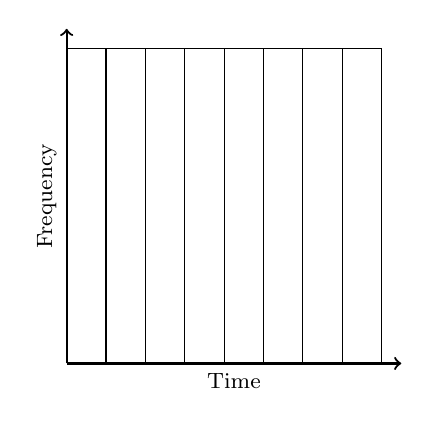
\begin{tikzpicture}
	\draw (0,0) -- (4,0);
	\draw (4,0) -- (4,-4);
	\path[thick, ->]  (0,-4) edge node[below] {\footnotesize Time} (4.25,-4)  ;
	\path[thick, ->] (0,-4) edge node[above, rotate=90] {\footnotesize Frequency} (0,.25)  ;
	
	\draw (.5,0) -- (.5,-4);
	\draw (1,0) -- (1,-4);
	\draw (1.5,0) -- (1.5,-4);
	\draw (2,0) -- (2,-4);
	\draw (2.5,0) -- (2.5,-4);
	\draw (3,0) -- (3,-4);
	\draw (3.5,0) -- (3.5,-4);
	\end{tikzpicture}
	\caption{Waveform}
\end{subfigure}%
\begin{subfigure}{.4\textwidth}
	\centering
	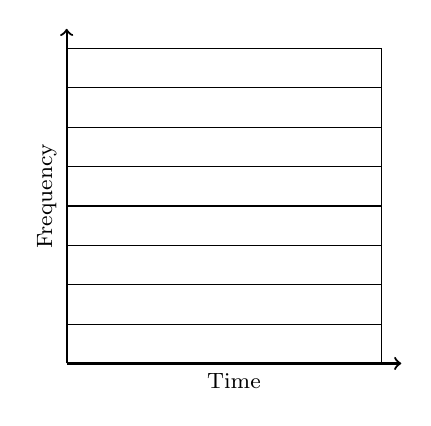
\begin{tikzpicture}
	\draw (0,0) -- (4,0);
	\draw (4,0) -- (4,-4);
	\path[thick, ->]  (0,-4) edge node[below] {\footnotesize Time} (4.25,-4)  ;
	\path[thick, ->] (0,-4) edge node[above, rotate=90] {\footnotesize Frequency} (0,.25)  ;
	
	\draw (0,-.5) -- (4,-.5);
	\draw (0,-1) -- (4,-1);
	\draw (0,-1.5) -- (4,-1.5);
	\draw (0,-2) -- (4,-2);
	\draw (0,-2.5) -- (4,-2.5);
	\draw (0,-3) -- (4,-3);
	\draw (0,-3.5) -- (4,-3.5);
	\end{tikzpicture}
	\caption{Fourier Transform}
\end{subfigure}

\medskip

\begin{subfigure}{.4\textwidth}
	\centering
		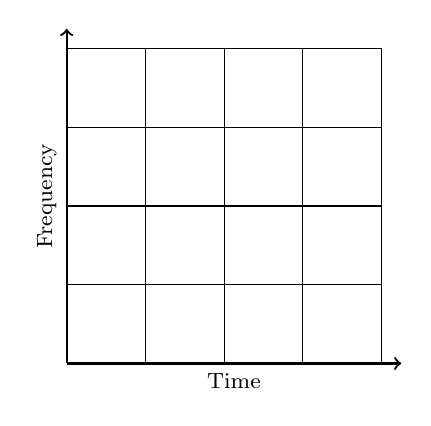
\begin{tikzpicture}
	
	\draw (0,0) -- (4,0);
	\draw (4,0) -- (4,-4);
	\path[thick, ->]  (0,-4) edge node[below] {\footnotesize Time} (4.25,-4)  ;
	\path[thick, ->] (0,-4) edge node[above, rotate=90] {\footnotesize Frequency} (0,.25)  ;
	
	\draw (1,0) -- (1,-4);
	\draw (0,-1) -- (4,-1);
	\draw (2,0) -- (2,-4);
	\draw (0,-2) -- (4,-2);
	\draw (3,0) -- (3,-4);
	\draw (0,-3) -- (4,-3);
	
	\end{tikzpicture}
	\caption{Short-Time Fourier Transform}
\end{subfigure}%
\begin{subfigure}{.4\textwidth}
	\centering
	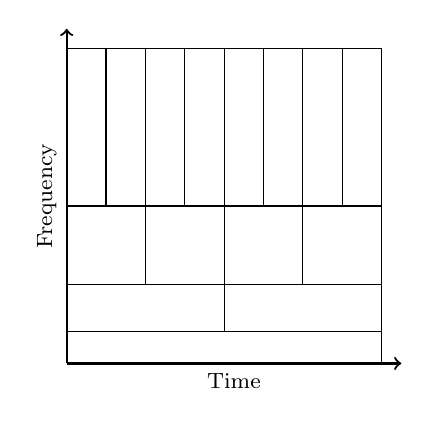
\begin{tikzpicture}
		\draw (0,0) -- (4,0);
		\draw (4,0) -- (4,-4);
		\path[thick, ->]  (0,-4) edge node[below] {\footnotesize Time} (4.25,-4)  ;
		\path[thick, ->] (0,-4) edge node[above, rotate=90] {\footnotesize Frequency} (0,.25)  ;
		\draw (0,-2) -- (4,-2);
		\draw (0,-3) -- (4,-3);
	
		\draw (0,-3.6) -- (4,-3.6);
		\draw (2,0) -- (2,-3.6);
	
		\draw[-] (1,0) -- (1,-3);
		\draw[-] (3,0) -- (3,-3);
	
		\draw[-] (.5,0) -- (.5,-2);
		\draw[-] (1.5,0) -- (1.5,-2);
	
		\draw[-] (2.5,0) -- (2.5,-2);
		\draw[-] (3.5,0) -- (3.5,-2);
	\end{tikzpicture}
	\caption{Wavelet Transform}
\end{subfigure}
    \caption{Time—frequency resolution plane}
    \label{fig:time-frequency-plane}
\end{figure}

Il existe une grande variété d'ondelettes qui servent à différentes fins comme l'ondelette de Morlet, l'ondelettes de Daubechies et bien d'autres.

\begin{figure}[H]
    \centering
    \includegraphics{figures/wavelets.pdf}
    \caption{Les différents types d'ondelettes}
    \label{fig:wavelets}
\end{figure}

\subsection{Transformée en ondelettes continue}
Mathématiquement, la transformation en ondelettes continue est définie par l'équation \ref{equation:cwt}:

\begin{equation}
    CWT_x^\psi(\tau, s)=\frac{1}{\sqrt{|s|}}\int_{-\infty}^{\infty}x(t)\psi^* \left(\frac{t-\tau}{s}\right)dt
    \label{equation:cwt}
\end{equation}

Où $x(t)$ est le signal original, $\psi^*$ est une fonction appelée \textbf{l'ondelette mère} ; $s$ et $\tau$ sont les facteurs de \textbf{dilatation} et \textbf{translation} respectivement. Le signal original est multiplié par l'ondelette mère qui est mise à l'échelle en utilisant différents facteurs de dilatation puis translatée sur le signal.

La sortie de \acrshort{cwt} est un scaleogram comme celui de la figure \ref{fig:scaleogram} qui est un scaleogram (tracé de contour rempli) de données de vibrations sur une durée de 25ms :

\begin{figure}[H]
    \centering
    \includegraphics{figures/scaleogram.pdf}
    \caption{Scaleogram d'un échantillon de vibrations}
    \label{fig:scaleogram}
\end{figure}

Les axes x et y représentent respectivement le temps et la fréquence. Les différentes couleurs indiquent la hauteur (c'est-à-dire l'amplitude) de chaque fréquence (axe des y) à chaque instant-de-temps (axe des x), ce qui—différemment de la transformation de Fourier—fournit des informations sur les fréquences présentes dans le signal ainsi que sur les moments où ces fréquences sont présentes.

\subsection{Transformation en ondelettes discrète}

Dans des applications pratiques, la transformation en ondelettes discrètes (\acrlong{dwt}: \acrshort{dwt}) est implémentée comme une banque de filtres où le signal est passé à travers des filtres passe-bas et passe-haut pour obtenir des \textbf{approximation} et des \textbf{coefficients de décomposition}. La figure \ref{fig:dwt} montre un \acrshort{dwt} avec 2 niveaux de décomposition qui donne des coefficients d'approximation et de décomposition du 2ème ordre :

\begin{figure}[H]
    \centering
    \begin{tikzpicture}[cell/.style={rectangle,draw, thick,align=center, minimum size=2em,inner sep=5pt}, input/.style={->}]

\node[cell] at (0,0) (xn) {$x[n]$};

\node[cell] at (-1.5,-1.5) (lpf1) {$LPF$};
\node[cell] at (1.5,-1.5) (hpf1){$HPF$};

\node[cell] at (-1.5,-3) (A1) {A1};
\node[cell, below = 1em of hpf1]  (D1) {D1};

\node[cell, below left = 2em of A1] (lpf2) {$LPF$};
\node[cell, below right = 2em of A1] (hpf2){$HPF$};

\node[cell, below = 1em of lpf2]  (A2) {A2};
\node[cell, below = 1em of hpf2]  (D2) {D2};

\draw[->, >=angle 60] (xn) -- ++(0,-1em) -- ++(0,-0.75em) -| (lpf1);
\draw[->, >=angle 60] (xn) -- ++(0,-1em) -- ++(0,-0.75em) -| (hpf1);

\draw[->, >=angle 60] (lpf1) -- (A1);
\draw[->, >=angle 60] (hpf1) -- (D1);

\draw[->, >=angle 60] (A1) -- ++(0,-1em) -- ++(0,-0.8em) -| (lpf2);
\draw[->, >=angle 60] (A1) -- ++(0,-1em) -- ++(0,-0.8em) -| (hpf2);

\draw[->, >=angle 60] (lpf2) -- (A2);
\draw[->, >=angle 60] (hpf2) -- (D2);

\node[] at (3,-0.9) (coord1) {};
\node[] at (3,-3.25) (coord2) {};

\end{tikzpicture}
    \caption{Transformation en ondelettes discrètes (\acrshort{dwt}) comme banque de filtres}
    \label{fig:dwt}
\end{figure}

\acrshort{dwt} donne deux séries de coefficients : \textbf{coefficients d'approximation} associé au filtre passe-bas et \textbf{coefficients de détail} associé au filtre passe-haut du \acrshort{dwt}. En appliquant à nouveau le \acrshort{dwt} sur les coefficients d'approximation, le niveau de décomposition suivant peut être obtenu. À chaque niveau, le signal original est sous-échantillonné d'un facteur 2, ce qui impose une limitation du nombre possible de niveaux de décomposition pour un signal donné.

\begin{figure}[H]
    \centering
    \includegraphics{figures/dwt_chirp.pdf}
    \caption{Décomposition du signal de niveau 3 à l'aide de \acrshort{dwt}}
    \label{fig:dwt-chirp-signal}
\end{figure}



\section{Conclusion}
Les données de vibration sont des signaux discrets échantillonnés à une certaine fréquence dans le temps. Bien qu'elles contiennent de nombreuses informations précieuses sur les performances des équipements, ces informations ne sont généralement pas directement observables dans le domaine temporel. Les techniques de traitement numérique du signal permettent de mieux comprendre les données brutes de vibration en les convertissant en domaines de fréquence ou de temps-fréquence où des composantes de fréquence inhabituelles peuvent indiquer le développement d'un certain modèle de dégradation. Ce chapitre a présenté plusieurs de ces techniques comme les transformations de Fourier et d'ondelettes. Un chapitre suivant présentera l'utilisation de ces techniques pour extraire des caractéristiques qui servent d'entrée pour un réseau de neurones qui peut estimer la durée de vie utile restante.







\begin{comment}
\chapterintrobox{Feature extraction is an important preprocessing step in the workflow of developing machine learning models and directly influences the model's performance. Therefore, this step should be carried out carefuly in order to extract meaningful features from the raw data. Vibration data carries very useful information about the system health, yet it needs a lot of preprocessing before being used as an input for a specific model. This chapter describes some of signal processing techniques used in traditional vibration analysis, but in this context they will be used as feature extractors for a neural network architecture.}

\section{Signal processing for vibration analysis}
Vibration data is vital for health assessment of a given system and carries out very useful information about its performance (refer to section \ref{sec:data-acquisition} for details about data acquisition), yet these information are usually hard to observe in its raw waveform. Signal processing techniques are used to convert the raw waveform from time domain into frequency or time–frequnecy domains.

\section{Fourier analysis}
Fourier analysis, also called harmonic analysis, of a periodic signal $x(t)$ is the decomposition of the series into summation of sinusoidal components, where each sinusoid has a specific amplitude and phase.

The Fourier transform (FT) of a signal $x(t)$ can be mathematically given by equation \ref{equation:fourier-transform}:

\begin{equation}
    X(w) = \int_{-\infty}^{\infty}x(n)e^{-jwt}dt
    \label{equation:fourier-transform}
\end{equation}

In practical applications of digital signal processing where signals are discrete in time rather than continuous (e.g. vibration analysis) a discretized version called discrete fourier transform (DFT) is used instead, it is expressed mathematically by equation \ref{equation:discrete-fourier-transform}:

\begin{equation}
    X(w) = \sum_{-\infty}^{\infty}x(t)e^{-jwt}dt
    \label{equation:discrete-fourier-transform}
\end{equation}

Fast Fourier transform (FFT) is an effective algorithm used to implement DFT in computers. Figure \ref{figure:fft} shows a signal in its waveform (or time domain) and its corresponding spectrum (frequency domain) obtained using FFT algorithm. The spectrum shows the frequency components present in the signal:

\begin{figure}[H]
    \centering
    \includegraphics{figures/fft.pdf}
    \caption{Signal in the time domain and its fast Fourier transform}
    \label{figure:fft}
\end{figure}

\section{Wavelet transform}
Wavelet transform is also a spectral analysis tool, like Fourier transform. The main difference is that Fourier transform decomposes the signal into sinusoidal components, but wavelet transform decomposes it into a set of oscillatory functions called \textbf{wavelets}. Unlike sinusoids, wavelets are localized in time, thus wavelet transform doesn't only provide information about the frequency present in a signal but also the time of their occurence. Wavelet transform is a much better solution than Fourier transform when studying non-linear non-stationary signals (i.e. its frequency components vary with time).

Figure \ref{fig:time-frequency-plane} shows the difference in time and frequency resolutions between different methods. In the waveform, the signal has absolute resolution in time and zero resolution in frequency. Fourier transform on the contrary transforms the signal totally into the frequency domain, therefore it has absolute resolution in frequency but no resolution in time. Short-time Fourier transform is calculated identically to fourier transform but it is performed on separate segments of the original signal to preserve some resolution in time. Wavelet transform on the other hand exhibits a high time resolution for high frequencies and high frequency resolution for low frequencies:

\begin{figure}[H]
    \centering
    \begin{subfigure}{.4\textwidth}
	\centering
	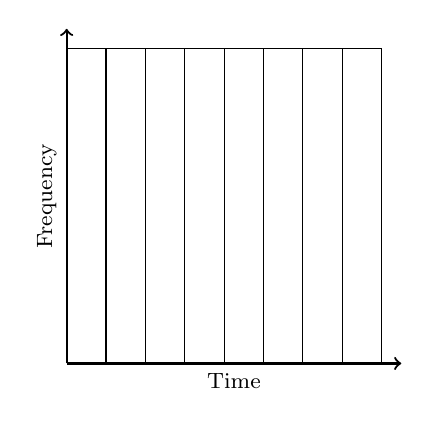
\begin{tikzpicture}
	\draw (0,0) -- (4,0);
	\draw (4,0) -- (4,-4);
	\path[thick, ->]  (0,-4) edge node[below] {\footnotesize Time} (4.25,-4)  ;
	\path[thick, ->] (0,-4) edge node[above, rotate=90] {\footnotesize Frequency} (0,.25)  ;
	
	\draw (.5,0) -- (.5,-4);
	\draw (1,0) -- (1,-4);
	\draw (1.5,0) -- (1.5,-4);
	\draw (2,0) -- (2,-4);
	\draw (2.5,0) -- (2.5,-4);
	\draw (3,0) -- (3,-4);
	\draw (3.5,0) -- (3.5,-4);
	\end{tikzpicture}
	\caption{Waveform}
\end{subfigure}%
\begin{subfigure}{.4\textwidth}
	\centering
	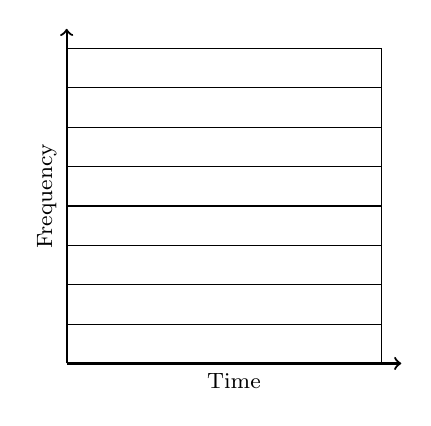
\begin{tikzpicture}
	\draw (0,0) -- (4,0);
	\draw (4,0) -- (4,-4);
	\path[thick, ->]  (0,-4) edge node[below] {\footnotesize Time} (4.25,-4)  ;
	\path[thick, ->] (0,-4) edge node[above, rotate=90] {\footnotesize Frequency} (0,.25)  ;
	
	\draw (0,-.5) -- (4,-.5);
	\draw (0,-1) -- (4,-1);
	\draw (0,-1.5) -- (4,-1.5);
	\draw (0,-2) -- (4,-2);
	\draw (0,-2.5) -- (4,-2.5);
	\draw (0,-3) -- (4,-3);
	\draw (0,-3.5) -- (4,-3.5);
	\end{tikzpicture}
	\caption{Fourier Transform}
\end{subfigure}

\medskip

\begin{subfigure}{.4\textwidth}
	\centering
		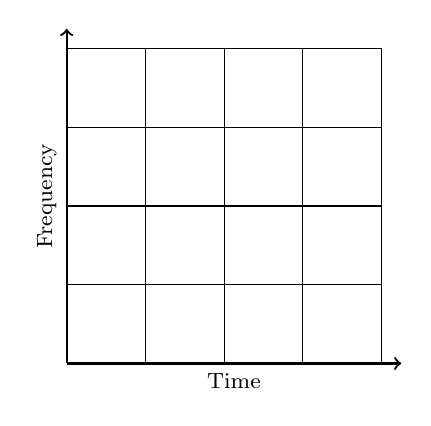
\begin{tikzpicture}
	
	\draw (0,0) -- (4,0);
	\draw (4,0) -- (4,-4);
	\path[thick, ->]  (0,-4) edge node[below] {\footnotesize Time} (4.25,-4)  ;
	\path[thick, ->] (0,-4) edge node[above, rotate=90] {\footnotesize Frequency} (0,.25)  ;
	
	\draw (1,0) -- (1,-4);
	\draw (0,-1) -- (4,-1);
	\draw (2,0) -- (2,-4);
	\draw (0,-2) -- (4,-2);
	\draw (3,0) -- (3,-4);
	\draw (0,-3) -- (4,-3);
	
	\end{tikzpicture}
	\caption{Short-Time Fourier Transform}
\end{subfigure}%
\begin{subfigure}{.4\textwidth}
	\centering
	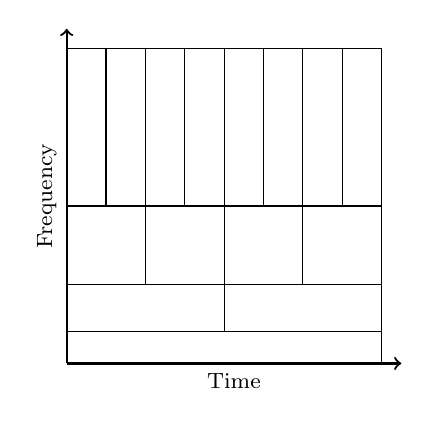
\begin{tikzpicture}
		\draw (0,0) -- (4,0);
		\draw (4,0) -- (4,-4);
		\path[thick, ->]  (0,-4) edge node[below] {\footnotesize Time} (4.25,-4)  ;
		\path[thick, ->] (0,-4) edge node[above, rotate=90] {\footnotesize Frequency} (0,.25)  ;
		\draw (0,-2) -- (4,-2);
		\draw (0,-3) -- (4,-3);
	
		\draw (0,-3.6) -- (4,-3.6);
		\draw (2,0) -- (2,-3.6);
	
		\draw[-] (1,0) -- (1,-3);
		\draw[-] (3,0) -- (3,-3);
	
		\draw[-] (.5,0) -- (.5,-2);
		\draw[-] (1.5,0) -- (1.5,-2);
	
		\draw[-] (2.5,0) -- (2.5,-2);
		\draw[-] (3.5,0) -- (3.5,-2);
	\end{tikzpicture}
	\caption{Wavelet Transform}
\end{subfigure}
    \caption{Time—frequency resolution plane}
    \label{fig:time-frequency-plane}
\end{figure}

There are a wide variety of wavelets that serve different purposes like Morlet wavelet, Daubechies wavelet and many others.

\begin{figure}[H]
    \centering
    \includegraphics{figures/wavelets.pdf}
    \caption{Different types of wavelets}
    \label{fig:wavelets}
\end{figure}

\subsection{Continuous wavelet transform}
Mathematically, continuous wavelet transform is defined by equation \ref{equation:cwt}:

\begin{equation}
    CWT_x^\psi(\tau, s)=\frac{1}{\sqrt{|s|}}\int_{-\infty}^{\infty}x(t)\psi^* \left(\frac{t-\tau}{s}\right)dt
    \label{equation:cwt}
\end{equation}

Where $x(t)$ is the original signal, $\psi^*$ is a function called the \textbf{mother wavelet}; $s$ and $\tau$ are the \textbf{scale} and \textbf{translation} parameters respectively. The original signal is multiplied by the mother wavelet which is scaled using different scales then translated over the signal.

The output of \acrshort{cwt} is a scaleogram like the one in figure \ref{fig:scaleogram} which is a scaleogram (filled contour plot) of vibrations data snapshot of 25ms:

\begin{figure}[H]
    \centering
    \includegraphics{figures/scaleogram.pdf}
    \caption{Scaleogram of vibration data snapshot}
    \label{fig:scaleogram}
\end{figure}

The x and y axes represent time and frequency respectively. Different colors indicate the power (i.e. amplitude) of each frequency (y-axis) during each instant of time (x-axis) which—unlike Fourier transform—provides information about the frequencies present in the signal and also the instances of time when these frequencies are present.

\subsection{Discrete wavelet transform}
In practical applicaions, discrete wavelet transform (DWT) is implemented as a filter bank where the signal is passed therough low- and high-pass filters to obtain \textbf{approximation} and \textbf{decomposition coefficients}. Figure \ref{fig:dwt} shows a DWT with 2 levels of decomposition which yields 2nd order approximation and decomposition coefficients:

\begin{figure}[H]
    \centering
    \begin{tikzpicture}[cell/.style={rectangle,draw, thick,align=center, minimum size=2em,inner sep=5pt}, input/.style={->}]

\node[cell] at (0,0) (xn) {$x[n]$};

\node[cell] at (-1.5,-1.5) (lpf1) {$LPF$};
\node[cell] at (1.5,-1.5) (hpf1){$HPF$};

\node[cell] at (-1.5,-3) (A1) {A1};
\node[cell, below = 1em of hpf1]  (D1) {D1};

\node[cell, below left = 2em of A1] (lpf2) {$LPF$};
\node[cell, below right = 2em of A1] (hpf2){$HPF$};

\node[cell, below = 1em of lpf2]  (A2) {A2};
\node[cell, below = 1em of hpf2]  (D2) {D2};

\draw[->, >=angle 60] (xn) -- ++(0,-1em) -- ++(0,-0.75em) -| (lpf1);
\draw[->, >=angle 60] (xn) -- ++(0,-1em) -- ++(0,-0.75em) -| (hpf1);

\draw[->, >=angle 60] (lpf1) -- (A1);
\draw[->, >=angle 60] (hpf1) -- (D1);

\draw[->, >=angle 60] (A1) -- ++(0,-1em) -- ++(0,-0.8em) -| (lpf2);
\draw[->, >=angle 60] (A1) -- ++(0,-1em) -- ++(0,-0.8em) -| (hpf2);

\draw[->, >=angle 60] (lpf2) -- (A2);
\draw[->, >=angle 60] (hpf2) -- (D2);

\node[] at (3,-0.9) (coord1) {};
\node[] at (3,-3.25) (coord2) {};

\end{tikzpicture}
    \caption{Discrete wavelet transform (DWT) as a filter bank}
    \label{fig:dwt}
\end{figure}

\begin{figure}[H]
    \centering
    \includegraphics{figures/dwt_chirp.pdf}
    \caption{Level 3 signal decomposition using DWT}
    \label{fig:dwt-chirp-signal}
\end{figure}

DWT returns two sets of coefficients: \textbf{approximation coefficients} associated with the low pass filter and \textbf{detail coefficients} associated with the high pass filter of the DWT. By applying DWT again on the approximation coefficients the next level of decomposition can be obtained. At each level the original signal is downsampled by a factor of 2, this fact imposes a limitation on the possible number of decomposition levels for a given signal.

\section{Conclusion}
Vibration data are discrete signals sampled at a certain frequency in time. Although they hold so many valuable information about equipment performance, these information are usually not directly observable in the time domain. Digital signal processing techniques offer a way to gain more insights from raw vibration data by converting it to frequency or time–frequency domains where unusual frequency components can indicate development of certain degradation pattern. This chapter introduced several of these techniques like Fourier and Wavelet transforms. A following chapter will present the use of these techniques for extracting features that serve as an input for a neural network that can estimate the remaining useful life.
\end{comment}

